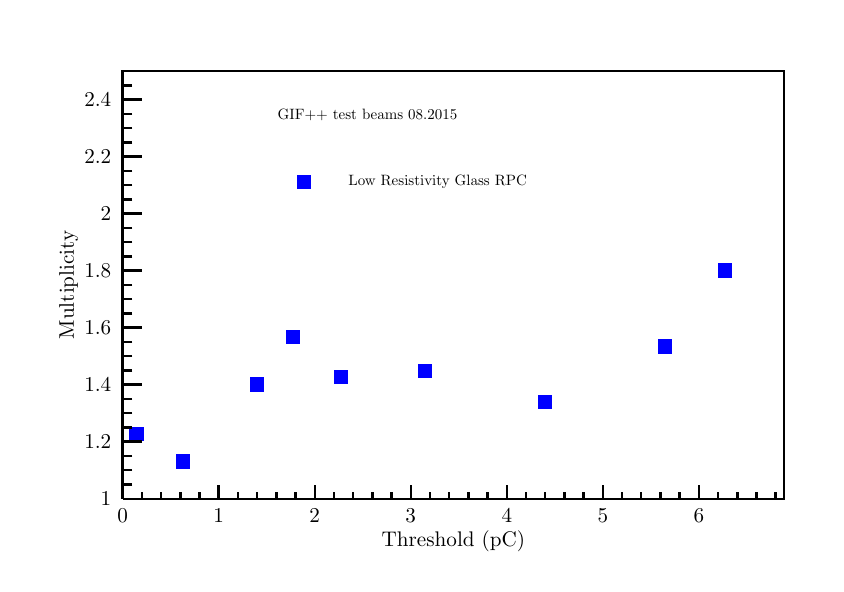
\begin{tikzpicture}
\pgfdeclareplotmark{cross} {
\pgfpathmoveto{\pgfpoint{-0.3\pgfplotmarksize}{\pgfplotmarksize}}
\pgfpathlineto{\pgfpoint{+0.3\pgfplotmarksize}{\pgfplotmarksize}}
\pgfpathlineto{\pgfpoint{+0.3\pgfplotmarksize}{0.3\pgfplotmarksize}}
\pgfpathlineto{\pgfpoint{+1\pgfplotmarksize}{0.3\pgfplotmarksize}}
\pgfpathlineto{\pgfpoint{+1\pgfplotmarksize}{-0.3\pgfplotmarksize}}
\pgfpathlineto{\pgfpoint{+0.3\pgfplotmarksize}{-0.3\pgfplotmarksize}}
\pgfpathlineto{\pgfpoint{+0.3\pgfplotmarksize}{-1.\pgfplotmarksize}}
\pgfpathlineto{\pgfpoint{-0.3\pgfplotmarksize}{-1.\pgfplotmarksize}}
\pgfpathlineto{\pgfpoint{-0.3\pgfplotmarksize}{-0.3\pgfplotmarksize}}
\pgfpathlineto{\pgfpoint{-1.\pgfplotmarksize}{-0.3\pgfplotmarksize}}
\pgfpathlineto{\pgfpoint{-1.\pgfplotmarksize}{0.3\pgfplotmarksize}}
\pgfpathlineto{\pgfpoint{-0.3\pgfplotmarksize}{0.3\pgfplotmarksize}}
\pgfpathclose
\pgfusepathqstroke
}
\pgfdeclareplotmark{cross*} {
\pgfpathmoveto{\pgfpoint{-0.3\pgfplotmarksize}{\pgfplotmarksize}}
\pgfpathlineto{\pgfpoint{+0.3\pgfplotmarksize}{\pgfplotmarksize}}
\pgfpathlineto{\pgfpoint{+0.3\pgfplotmarksize}{0.3\pgfplotmarksize}}
\pgfpathlineto{\pgfpoint{+1\pgfplotmarksize}{0.3\pgfplotmarksize}}
\pgfpathlineto{\pgfpoint{+1\pgfplotmarksize}{-0.3\pgfplotmarksize}}
\pgfpathlineto{\pgfpoint{+0.3\pgfplotmarksize}{-0.3\pgfplotmarksize}}
\pgfpathlineto{\pgfpoint{+0.3\pgfplotmarksize}{-1.\pgfplotmarksize}}
\pgfpathlineto{\pgfpoint{-0.3\pgfplotmarksize}{-1.\pgfplotmarksize}}
\pgfpathlineto{\pgfpoint{-0.3\pgfplotmarksize}{-0.3\pgfplotmarksize}}
\pgfpathlineto{\pgfpoint{-1.\pgfplotmarksize}{-0.3\pgfplotmarksize}}
\pgfpathlineto{\pgfpoint{-1.\pgfplotmarksize}{0.3\pgfplotmarksize}}
\pgfpathlineto{\pgfpoint{-0.3\pgfplotmarksize}{0.3\pgfplotmarksize}}
\pgfpathclose
\pgfusepathqfillstroke
}
\pgfdeclareplotmark{newstar} {
\pgfpathmoveto{\pgfqpoint{0pt}{\pgfplotmarksize}}
\pgfpathlineto{\pgfqpointpolar{44}{0.5\pgfplotmarksize}}
\pgfpathlineto{\pgfqpointpolar{18}{\pgfplotmarksize}}
\pgfpathlineto{\pgfqpointpolar{-20}{0.5\pgfplotmarksize}}
\pgfpathlineto{\pgfqpointpolar{-54}{\pgfplotmarksize}}
\pgfpathlineto{\pgfqpointpolar{-90}{0.5\pgfplotmarksize}}
\pgfpathlineto{\pgfqpointpolar{234}{\pgfplotmarksize}}
\pgfpathlineto{\pgfqpointpolar{198}{0.5\pgfplotmarksize}}
\pgfpathlineto{\pgfqpointpolar{162}{\pgfplotmarksize}}
\pgfpathlineto{\pgfqpointpolar{134}{0.5\pgfplotmarksize}}
\pgfpathclose
\pgfusepathqstroke
}
\pgfdeclareplotmark{newstar*} {
\pgfpathmoveto{\pgfqpoint{0pt}{\pgfplotmarksize}}
\pgfpathlineto{\pgfqpointpolar{44}{0.5\pgfplotmarksize}}
\pgfpathlineto{\pgfqpointpolar{18}{\pgfplotmarksize}}
\pgfpathlineto{\pgfqpointpolar{-20}{0.5\pgfplotmarksize}}
\pgfpathlineto{\pgfqpointpolar{-54}{\pgfplotmarksize}}
\pgfpathlineto{\pgfqpointpolar{-90}{0.5\pgfplotmarksize}}
\pgfpathlineto{\pgfqpointpolar{234}{\pgfplotmarksize}}
\pgfpathlineto{\pgfqpointpolar{198}{0.5\pgfplotmarksize}}
\pgfpathlineto{\pgfqpointpolar{162}{\pgfplotmarksize}}
\pgfpathlineto{\pgfqpointpolar{134}{0.5\pgfplotmarksize}}
\pgfpathclose
\pgfusepathqfillstroke
}
\definecolor{c}{rgb}{1,1,1};
\draw [color=c, fill=c] (0,0) rectangle (10,6.79083);
\definecolor{c}{rgb}{0,0,0};
\draw [c,line width=0.9] (1.2,0.8149) -- (1.2,6.24756) -- (9.6,6.24756) -- (9.6,0.8149) -- (1.2,0.8149);
\draw [c,line width=0.9] (1.2,0.8149) -- (1.2,6.24756) -- (9.6,6.24756) -- (9.6,0.8149) -- (1.2,0.8149);
\draw [c,line width=0.9] (1.2,0.8149) -- (1.2,6.24756) -- (9.6,6.24756) -- (9.6,0.8149) -- (1.2,0.8149);
\draw [c,line width=0.9] (1.2,0.8149) -- (1.2,6.24756) -- (9.6,6.24756) -- (9.6,0.8149) -- (1.2,0.8149);
\draw [c,line width=0.9] (1.2,0.8149) -- (9.6,0.8149);
\draw [c,line width=0.9] (1.2,0.986029) -- (1.2,0.8149);
\draw [c,line width=0.9] (1.44389,0.900464) -- (1.44389,0.8149);
\draw [c,line width=0.9] (1.68779,0.900464) -- (1.68779,0.8149);
\draw [c,line width=0.9] (1.93168,0.900464) -- (1.93168,0.8149);
\draw [c,line width=0.9] (2.17558,0.900464) -- (2.17558,0.8149);
\draw [c,line width=0.9] (2.41947,0.986029) -- (2.41947,0.8149);
\draw [c,line width=0.9] (2.66337,0.900464) -- (2.66337,0.8149);
\draw [c,line width=0.9] (2.90726,0.900464) -- (2.90726,0.8149);
\draw [c,line width=0.9] (3.15116,0.900464) -- (3.15116,0.8149);
\draw [c,line width=0.9] (3.39505,0.900464) -- (3.39505,0.8149);
\draw [c,line width=0.9] (3.63895,0.986029) -- (3.63895,0.8149);
\draw [c,line width=0.9] (3.88284,0.900464) -- (3.88284,0.8149);
\draw [c,line width=0.9] (4.12674,0.900464) -- (4.12674,0.8149);
\draw [c,line width=0.9] (4.37063,0.900464) -- (4.37063,0.8149);
\draw [c,line width=0.9] (4.61453,0.900464) -- (4.61453,0.8149);
\draw [c,line width=0.9] (4.85842,0.986029) -- (4.85842,0.8149);
\draw [c,line width=0.9] (5.10232,0.900464) -- (5.10232,0.8149);
\draw [c,line width=0.9] (5.34621,0.900464) -- (5.34621,0.8149);
\draw [c,line width=0.9] (5.59011,0.900464) -- (5.59011,0.8149);
\draw [c,line width=0.9] (5.834,0.900464) -- (5.834,0.8149);
\draw [c,line width=0.9] (6.0779,0.986029) -- (6.0779,0.8149);
\draw [c,line width=0.9] (6.32179,0.900464) -- (6.32179,0.8149);
\draw [c,line width=0.9] (6.56569,0.900464) -- (6.56569,0.8149);
\draw [c,line width=0.9] (6.80958,0.900464) -- (6.80958,0.8149);
\draw [c,line width=0.9] (7.05348,0.900464) -- (7.05348,0.8149);
\draw [c,line width=0.9] (7.29737,0.986029) -- (7.29737,0.8149);
\draw [c,line width=0.9] (7.54127,0.900464) -- (7.54127,0.8149);
\draw [c,line width=0.9] (7.78516,0.900464) -- (7.78516,0.8149);
\draw [c,line width=0.9] (8.02906,0.900464) -- (8.02906,0.8149);
\draw [c,line width=0.9] (8.27295,0.900464) -- (8.27295,0.8149);
\draw [c,line width=0.9] (8.51685,0.986029) -- (8.51685,0.8149);
\draw [c,line width=0.9] (8.51685,0.986029) -- (8.51685,0.8149);
\draw [c,line width=0.9] (8.76074,0.900464) -- (8.76074,0.8149);
\draw [c,line width=0.9] (9.00464,0.900464) -- (9.00464,0.8149);
\draw [c,line width=0.9] (9.24853,0.900464) -- (9.24853,0.8149);
\draw [c,line width=0.9] (9.49242,0.900464) -- (9.49242,0.8149);
\draw [anchor=base] (1.2,0.509312) node[scale=0.763657, color=c, rotate=0]{0};
\draw [anchor=base] (2.41947,0.509312) node[scale=0.763657, color=c, rotate=0]{1};
\draw [anchor=base] (3.63895,0.509312) node[scale=0.763657, color=c, rotate=0]{2};
\draw [anchor=base] (4.85842,0.509312) node[scale=0.763657, color=c, rotate=0]{3};
\draw [anchor=base] (6.0779,0.509312) node[scale=0.763657, color=c, rotate=0]{4};
\draw [anchor=base] (7.29737,0.509312) node[scale=0.763657, color=c, rotate=0]{5};
\draw [anchor=base] (8.51685,0.509312) node[scale=0.763657, color=c, rotate=0]{6};
\draw (5.4,0.271633) node[scale=0.763657, color=c, rotate=0]{Threshold (pC)};
\draw [c,line width=0.9] (1.2,0.8149) -- (1.2,6.24756);
\draw [c,line width=0.9] (1.44,0.8149) -- (1.2,0.8149);
\draw [c,line width=0.9] (1.32,0.995989) -- (1.2,0.995989);
\draw [c,line width=0.9] (1.32,1.17708) -- (1.2,1.17708);
\draw [c,line width=0.9] (1.32,1.35817) -- (1.2,1.35817);
\draw [c,line width=0.9] (1.44,1.53926) -- (1.2,1.53926);
\draw [c,line width=0.9] (1.32,1.72034) -- (1.2,1.72034);
\draw [c,line width=0.9] (1.32,1.90143) -- (1.2,1.90143);
\draw [c,line width=0.9] (1.32,2.08252) -- (1.2,2.08252);
\draw [c,line width=0.9] (1.44,2.26361) -- (1.2,2.26361);
\draw [c,line width=0.9] (1.32,2.4447) -- (1.2,2.4447);
\draw [c,line width=0.9] (1.32,2.62579) -- (1.2,2.62579);
\draw [c,line width=0.9] (1.32,2.80688) -- (1.2,2.80688);
\draw [c,line width=0.9] (1.44,2.98797) -- (1.2,2.98797);
\draw [c,line width=0.9] (1.32,3.16905) -- (1.2,3.16905);
\draw [c,line width=0.9] (1.32,3.35014) -- (1.2,3.35014);
\draw [c,line width=0.9] (1.32,3.53123) -- (1.2,3.53123);
\draw [c,line width=0.9] (1.44,3.71232) -- (1.2,3.71232);
\draw [c,line width=0.9] (1.32,3.89341) -- (1.2,3.89341);
\draw [c,line width=0.9] (1.32,4.0745) -- (1.2,4.0745);
\draw [c,line width=0.9] (1.32,4.25559) -- (1.2,4.25559);
\draw [c,line width=0.9] (1.44,4.43668) -- (1.2,4.43668);
\draw [c,line width=0.9] (1.32,4.61776) -- (1.2,4.61776);
\draw [c,line width=0.9] (1.32,4.79885) -- (1.2,4.79885);
\draw [c,line width=0.9] (1.32,4.97994) -- (1.2,4.97994);
\draw [c,line width=0.9] (1.44,5.16103) -- (1.2,5.16103);
\draw [c,line width=0.9] (1.32,5.34212) -- (1.2,5.34212);
\draw [c,line width=0.9] (1.32,5.52321) -- (1.2,5.52321);
\draw [c,line width=0.9] (1.32,5.7043) -- (1.2,5.7043);
\draw [c,line width=0.9] (1.44,5.88539) -- (1.2,5.88539);
\draw [c,line width=0.9] (1.44,5.88539) -- (1.2,5.88539);
\draw [c,line width=0.9] (1.32,6.06648) -- (1.2,6.06648);
\draw [c,line width=0.9] (1.32,6.24756) -- (1.2,6.24756);
\draw [anchor= east] (1.15,0.8149) node[scale=0.763657, color=c, rotate=0]{1};
\draw [anchor= east] (1.15,1.53926) node[scale=0.763657, color=c, rotate=0]{1.2};
\draw [anchor= east] (1.15,2.26361) node[scale=0.763657, color=c, rotate=0]{1.4};
\draw [anchor= east] (1.15,2.98797) node[scale=0.763657, color=c, rotate=0]{1.6};
\draw [anchor= east] (1.15,3.71232) node[scale=0.763657, color=c, rotate=0]{1.8};
\draw [anchor= east] (1.15,4.43668) node[scale=0.763657, color=c, rotate=0]{2};
\draw [anchor= east] (1.15,5.16103) node[scale=0.763657, color=c, rotate=0]{2.2};
\draw [anchor= east] (1.15,5.88539) node[scale=0.763657, color=c, rotate=0]{2.4};
\draw (0.512321,3.53123) node[scale=0.763657, color=c, rotate=90]{Multiplicity};
\definecolor{c}{rgb}{0,0,1};
\foreach \P in {(1.37421,1.63494), (1.96652,1.28729), (2.90726,2.26361), (3.36457,2.86903), (3.9743,2.35861), (5.04134,2.441), (6.56569,2.04493), (8.09003,2.7465), (8.8522,3.71232)}{\draw[mark options={color=c,fill=c},mark
 size=2.402402pt,mark=square*] plot coordinates {\P};}
\definecolor{c}{rgb}{1,1,1};
\draw [color=c, fill=c] (3,4.41404) rectangle (7,6.11175);
\definecolor{c}{rgb}{0,0,0};
\draw [anchor= west] (3.1,5.68732) node[scale=0.540924, color=c, rotate=0]{GIF++ test beams 08.2015};
\draw [anchor= west] (4,4.83847) node[scale=0.540924, color=c, rotate=0]{Low Resistivity Glass RPC};
\definecolor{c}{rgb}{0,0,1};
\foreach \P in {(3.5,4.83847)}{\draw[mark options={color=c,fill=c},mark size=2.402402pt,mark=square*] plot coordinates {\P};}
\definecolor{c}{rgb}{0,0,0};
\draw [c,line width=0.9] (1.2,0.8149) -- (9.6,0.8149);
\draw [c,line width=0.9] (1.2,0.986029) -- (1.2,0.8149);
\draw [c,line width=0.9] (1.44389,0.900464) -- (1.44389,0.8149);
\draw [c,line width=0.9] (1.68779,0.900464) -- (1.68779,0.8149);
\draw [c,line width=0.9] (1.93168,0.900464) -- (1.93168,0.8149);
\draw [c,line width=0.9] (2.17558,0.900464) -- (2.17558,0.8149);
\draw [c,line width=0.9] (2.41947,0.986029) -- (2.41947,0.8149);
\draw [c,line width=0.9] (2.66337,0.900464) -- (2.66337,0.8149);
\draw [c,line width=0.9] (2.90726,0.900464) -- (2.90726,0.8149);
\draw [c,line width=0.9] (3.15116,0.900464) -- (3.15116,0.8149);
\draw [c,line width=0.9] (3.39505,0.900464) -- (3.39505,0.8149);
\draw [c,line width=0.9] (3.63895,0.986029) -- (3.63895,0.8149);
\draw [c,line width=0.9] (3.88284,0.900464) -- (3.88284,0.8149);
\draw [c,line width=0.9] (4.12674,0.900464) -- (4.12674,0.8149);
\draw [c,line width=0.9] (4.37063,0.900464) -- (4.37063,0.8149);
\draw [c,line width=0.9] (4.61453,0.900464) -- (4.61453,0.8149);
\draw [c,line width=0.9] (4.85842,0.986029) -- (4.85842,0.8149);
\draw [c,line width=0.9] (5.10232,0.900464) -- (5.10232,0.8149);
\draw [c,line width=0.9] (5.34621,0.900464) -- (5.34621,0.8149);
\draw [c,line width=0.9] (5.59011,0.900464) -- (5.59011,0.8149);
\draw [c,line width=0.9] (5.834,0.900464) -- (5.834,0.8149);
\draw [c,line width=0.9] (6.0779,0.986029) -- (6.0779,0.8149);
\draw [c,line width=0.9] (6.32179,0.900464) -- (6.32179,0.8149);
\draw [c,line width=0.9] (6.56569,0.900464) -- (6.56569,0.8149);
\draw [c,line width=0.9] (6.80958,0.900464) -- (6.80958,0.8149);
\draw [c,line width=0.9] (7.05348,0.900464) -- (7.05348,0.8149);
\draw [c,line width=0.9] (7.29737,0.986029) -- (7.29737,0.8149);
\draw [c,line width=0.9] (7.54127,0.900464) -- (7.54127,0.8149);
\draw [c,line width=0.9] (7.78516,0.900464) -- (7.78516,0.8149);
\draw [c,line width=0.9] (8.02906,0.900464) -- (8.02906,0.8149);
\draw [c,line width=0.9] (8.27295,0.900464) -- (8.27295,0.8149);
\draw [c,line width=0.9] (8.51685,0.986029) -- (8.51685,0.8149);
\draw [c,line width=0.9] (8.51685,0.986029) -- (8.51685,0.8149);
\draw [c,line width=0.9] (8.76074,0.900464) -- (8.76074,0.8149);
\draw [c,line width=0.9] (9.00464,0.900464) -- (9.00464,0.8149);
\draw [c,line width=0.9] (9.24853,0.900464) -- (9.24853,0.8149);
\draw [c,line width=0.9] (9.49242,0.900464) -- (9.49242,0.8149);
\draw [c,line width=0.9] (1.2,0.8149) -- (1.2,6.24756);
\draw [c,line width=0.9] (1.44,0.8149) -- (1.2,0.8149);
\draw [c,line width=0.9] (1.32,0.995989) -- (1.2,0.995989);
\draw [c,line width=0.9] (1.32,1.17708) -- (1.2,1.17708);
\draw [c,line width=0.9] (1.32,1.35817) -- (1.2,1.35817);
\draw [c,line width=0.9] (1.44,1.53926) -- (1.2,1.53926);
\draw [c,line width=0.9] (1.32,1.72034) -- (1.2,1.72034);
\draw [c,line width=0.9] (1.32,1.90143) -- (1.2,1.90143);
\draw [c,line width=0.9] (1.32,2.08252) -- (1.2,2.08252);
\draw [c,line width=0.9] (1.44,2.26361) -- (1.2,2.26361);
\draw [c,line width=0.9] (1.32,2.4447) -- (1.2,2.4447);
\draw [c,line width=0.9] (1.32,2.62579) -- (1.2,2.62579);
\draw [c,line width=0.9] (1.32,2.80688) -- (1.2,2.80688);
\draw [c,line width=0.9] (1.44,2.98797) -- (1.2,2.98797);
\draw [c,line width=0.9] (1.32,3.16905) -- (1.2,3.16905);
\draw [c,line width=0.9] (1.32,3.35014) -- (1.2,3.35014);
\draw [c,line width=0.9] (1.32,3.53123) -- (1.2,3.53123);
\draw [c,line width=0.9] (1.44,3.71232) -- (1.2,3.71232);
\draw [c,line width=0.9] (1.32,3.89341) -- (1.2,3.89341);
\draw [c,line width=0.9] (1.32,4.0745) -- (1.2,4.0745);
\draw [c,line width=0.9] (1.32,4.25559) -- (1.2,4.25559);
\draw [c,line width=0.9] (1.44,4.43668) -- (1.2,4.43668);
\draw [c,line width=0.9] (1.32,4.61776) -- (1.2,4.61776);
\draw [c,line width=0.9] (1.32,4.79885) -- (1.2,4.79885);
\draw [c,line width=0.9] (1.32,4.97994) -- (1.2,4.97994);
\draw [c,line width=0.9] (1.44,5.16103) -- (1.2,5.16103);
\draw [c,line width=0.9] (1.32,5.34212) -- (1.2,5.34212);
\draw [c,line width=0.9] (1.32,5.52321) -- (1.2,5.52321);
\draw [c,line width=0.9] (1.32,5.7043) -- (1.2,5.7043);
\draw [c,line width=0.9] (1.44,5.88539) -- (1.2,5.88539);
\draw [c,line width=0.9] (1.44,5.88539) -- (1.2,5.88539);
\draw [c,line width=0.9] (1.32,6.06648) -- (1.2,6.06648);
\draw [c,line width=0.9] (1.32,6.24756) -- (1.2,6.24756);
\draw [c,line width=0.9] (1.2,0.8149) -- (1.2,6.24756) -- (9.6,6.24756) -- (9.6,0.8149) -- (1.2,0.8149);
\draw [c,line width=0.9] (1.2,0.8149) -- (1.2,6.24756) -- (9.6,6.24756) -- (9.6,0.8149) -- (1.2,0.8149);
\end{tikzpicture}
